%%%%%%%%%%%%%%%%%%%%%%% file template.tex %%%%%%%%%%%%%%%%%%%%%%%%%
%
% This is a general template file for the LaTeX package SVJour3
% for Springer journals.          Springer Heidelberg 2010/09/16
%
% Copy it to a new file with a new name and use it as the basis
% for your article. Delete % signs as needed.
%
% This template includes a few options for different layouts and
% content for various journals. Please consult a previous issue of
% your journal as needed.
%
%%%%%%%%%%%%%%%%%%%%%%%%%%%%%%%%%%%%%%%%%%%%%%%%%%%%%%%%%%%%%%%%%%%
%
% First comes an example EPS file -- just ignore it and
% proceed on the \documentclass line
% your LaTeX will extract the file if required
\begin{filecontents*}{example.eps}
%!PS-Adobe-3.0 EPSF-3.0
%%BoundingBox: 19 19 221 221
%%CreationDate: Mon Sep 29 1997
%%Creator: programmed by hand (JK)
%%EndComments
gsave
newpath
  20 20 moveto
  20 220 lineto
  220 220 lineto
  220 20 lineto
closepath
2 setlinewidth
gsave
  .4 setgray fill
grestore
stroke
grestore
\end{filecontents*}
%
\RequirePackage{fix-cm}
%
%\documentclass{svjour3}                     % onecolumn (standard format)
%\documentclass[smallcondensed]{svjour3}     % onecolumn (ditto)
\documentclass[smallextended]{svjour3}       % onecolumn (second format)
%\documentclass[twocolumn]{svjour3}          % twocolumn
%
\smartqed  % flush right qed marks, e.g. at end of proof
%
\usepackage{graphicx}
\usepackage{natbib}
\usepackage{booktabs}
\usepackage{algorithm}
\usepackage{algpseudocode}
%
% \usepackage{mathptmx}      % use Times fonts if available on your TeX system
%
% insert here the call for the packages your document requires
%\usepackage{latexsym}
% etc.
%
% please place your own definitions here and don't use \def but
% \newcommand{}{}
%
% Insert the name of "your journal" with
% \journalname{myjournal}
%
\begin{document}

\title{Evolving Mean-Update Selection Methods for CMA-ES}%\thanks{Grants or other notes
%about the article that should go on the front page should be
%placed here. General acknowledgments should be placed at the end of the article.}
%}

%\titlerunning{Evolving Mean-Update Selection Methods for CMA-ES}        % if too long for running head

\author{Samuel N. Richter          \and
        Michael Schoen             \and 
        Daniel R. Tauritz
}

%\authorrunning{Short form of author list} % if too long for running head

\institute{Samuel N. Richter \at
              Missouri University of Science and Technology \\ Natural Computation Lab
              \email{snr359@mst.edu}           %  \\
%             \emph{Present address:} of F. Author  %  if needed
           \and
           Michael G. Schoen \at
              Missouri University of Science and Technology \\ Natural Computation Lab
              \email{ms778@mst.edu} 
           \and
           Daniel R. Tauritz \at
              Missouri University of Science and Technology \\ Natural Computation Lab
              \email{dtauritz@acm.org} 
}

\date{Received: date / Accepted: date}
% The correct dates will be entered by the editor


\maketitle

\begin{abstract}
Selection functions enable Evolutionary Algorithms (EAs) to apply selection pressure to a population of individuals, whether by directly making decisions on whether an individual’s genes survive, or by selecting the individuals used to update the internal variables of the EA and thus influencing its behavior. Various conventional selection functions exist, each providing a unique method of selecting individuals, typically based on fitness. However, the full space of selection functions is effectively unlimited in size, and each possible selection algorithm is optimal for some EA configuration applied to a particular function class. Therefore, improved performance can be obtained by tuning selection functions to the problem at hand, rather than employing conventional selection functions. This paper details an investigation of the extent to which performance can be improved for the Covariance Matrix Adaptation Evolution Strategy (CMA-ES) by tuning the selection of individuals used for the mean-update algorithm. A hyper-heuristic is employed to explore the space of algorithms which select individuals from the population. We show the increase in performance obtained with a tuned selection algorithm, versus the unmodified CMA-ES mean-update algorithm. Specifically, we measure performance on instances from several real-valued benchmark function classes to demonstrate generalization of the improved performance.
\keywords{First keyword \and Second keyword \and More}
% \PACS{PACS code1 \and PACS code2 \and more}
% \subclass{MSC code1 \and MSC code2 \and more}
\end{abstract}

\section{Introduction}
\label{Introduction}
The performance of an Evolutionary Algorithm (EA) is highly sensitive to the parameters used to configure it~\citep{eiben1999parameter}. The field of automated algorithm design addresses this by exploring methods to remove the human bias in algorithm design and configuration. Hyper-heuristics, in particular, have been used to automate the generation of EA heuristics and algorithmic components, such as mutation operators, recombination operators, population sizing, and selection functions.

EAs employ selection functions to control the method by which an individual's genes are selected, for purposes such as, recombination, survival, or updating internal variables. Various conventional fitness-based selection functions exist, each providing a unique method of selecting individuals. These selected individuals may then undergo recombination and/or survival selection, or be used for some other update to the status of the population and internal variables of the EA. Often, the goal of these selection functions is to push the population of the EA towards an area of higher fitness, or to explore a region of the search space to find a potential growth direction. It follows that each selection algorithm plays a significant role in determining the behavior of the EA and the population, and thus, the average performance of the EA's search through the space of solutions~\citep{woodward2010metaBias}. Many selection algorithms are parameterized, allowing for further variance in the behavior they provide. In cases where parameterized selection algorithms are applied, the parameters can be carefully tuned, either manually or with tuning algorithms, to maximize the performance of an EA on a particular function or function class.

New selection algorithms can be designed in cases where the performance offered by existing algorithms is insufficient, even with well-tuned parameters. However, the full space of selection algorithms is effectively unlimited, and so it is highly unlikely that any conventionally human-designed algorithm offers the optimal selection behavior, given a specific problem. An implication of the ``No Free Lunch'' theorem~\citep{wolpert1995noFreeLunch} is that each possible selection algorithm is optimal for some EA configuration applied to a particular function class. Therefore, a performance gain is likely to be attained by exploring the space of selection algorithms to find one that offers better performance than any conventional selection algorithm. Previous work has confirmed this hypothesis, prompting our approach to use a hyper-heuristic and a custom representation of selection functions to explore the space of new selection functions ~\citep{woodward2011selection}.

Our approach employs a hyper-heuristic, with both generative and perturbative elements, to explore the space of selection algorithms, with each search algorithm represented by two components. The first component is a Koza-style Genetic Programming (GP) tree~\citep{koza1994genetic}, encoding a mathematical function that calculates how desirable an individual is at the current stage of evolution. The second component is a method of selecting individuals, based on how desirable they are calculated to be. We use this hyper-heuristic to evolve a new scheme for selecting individuals in the mean update function of the Covariance Matrix Adaptation Evolution Strategy (CMA-ES)~\citep{hansen1996cmaes}. The canonical CMA-ES has shown great success in solving a wide variety of problems, and given the improvement to a canonical EA via evolution of a new selection process shown in ~\citep{richter2018adpsea}, we sought to apply the same process to CMA-ES, anticipating a similar improvement.
\section{Related Work}
\label{Literature Review}
The field of hyper-heuristics encompasses many different approaches for the automated design of new algorithms. Methods may utilize offline learning, in which computation is done \textit{a priori} to develop a heuristic, or online learning, in which a heuristic is developed dynamically alongside a running problem. Hyper-heuristic searches can be perturbative, in which complete solutions are considered individually, or generative, in which solutions begin partially built and are extended iteratively~\citep{burke2013HHstateoftheart}. The hyper-heuristic presented in this paper is an offline-learning heuristic that combines these approaches, building one component of a selection algorithm with a generative method, and selecting another component in a perturbative manner.

A major application of hyper-heuristics is the automated design of algorithmic components, which various algorithms have been shown to benefit from. Hyper-heuristics have been used to evolve new algorithms from components of existing algorithms for Ant Colony optimization algorithms~\citep{lopez2012antcol}, Boolean Satisfiability solvers~\citep{khudabukhsh2009satenstein}, local search heuristics~\citep{burke2012localHeuristics}, and iterative parse trees representing Black Box Search Algorithms~\citep{martin2013evolvingBBSA}. The research described in this paper applies the same concept to selection functions, employing a hyper-heuristic to build selection functions from smaller components to search the space of new selection functions. In particular, the practice of using GP as a hyper-heuristic has been discussed in~\citep{burke2009exploring} and explored in a number of works~\citep{burke2010strippacking, burke2006binpacking, harris2015comparison}. 

Previous work has also focused on improvement of targeted components of EAs, including the evolution of new mutation operators~\citep{woodward2012mutationGeneration, hong2013probMutation}, mating preferences~\citep{guntly2011limp}, genetic representation of individuals~\citep{scott2015geneticRepresentations}, and crossover operators~\citep{goldman2011scc}. Methods for generating selection algorithms, in particular, have been investigated. A random walk through the space of register machines that compute and return a probability of selection for each individual showed that such custom-tuned selection algorithms can outperform typical selection algorithms~\citep{woodward2011selection}. A more informed search through the space of selection algorithms may yield an even greater benefit than a random search. In the previous work involving the evolution of Black Box Search Algorithms, the parse trees include evolved selection functions, although the selection functions are limited to two conventional selection functions (\textit{k}-tournament and truncation) with evolved parameters~\citep{martin2013evolvingBBSA}. An evolutionary search through selection functions developed with Grammatical Evolution showed that better selection functions can be developed using a hyper-heuristic, and that the performance of these selection functions can generalize to new instances within the same function class~\citep{lourencco2013selection}. A similar hyper-heuristic search employed GP to discover new selection algorithms, again showing a generalized increase in performance for the same EA running on the same problem set~\citep{richter2018adpsea}. The work described in this paper expands on these ideas by applying the hyper-heuristic search employing GP to the mean-update function of CMA-ES, changing the method used to select the population members used to update the mean in order to tune the performance of CMA-ES for a particular function class.

To search the space of selection algorithms defined by this representation, we employ a combination of perturbative and generative hyper-heuristics. Previous work has applied such combinations of hyper-heuristic types to memetic algorithms~\citep{krasnogor2004memetic}, EA operator control~\citep{maturana2010autonomous}, low-level heuristic management~\citep{remde2012empirical}, and vehicle routing~\citep{garrido2010vehicleRouting}. 
\section{Methodology}
\label{Methodology}
Here we discuss the methodology of our hyper-heuristic, and the meta-EA powering it. We first outline the format we use to represent selection functions in the meta-EA. The selection functions are built by a combined generative and perturbative hyper-heuristic. We then discuss how we use the meta-EA to evaluate and search for new selection functions. 
\subsection{Encoding Selection Functions}
\label{Methodology-Encoding Selection Functions}

Most typical selection functions are formatted as a series of algorithmic steps, which take as input a population of individuals and output a subset of the individuals, as selected by the algorithm. While we could explore the entire combinatorial space of algorithmic steps to find new selection functions, doing so would generate many algorithms which are not valid selection functions, or even functional algorithms. Therefore, we need a representation of selection functions that is both robust enough to represent a wide variety of selection functions, yet constrained enough that we can effectively search within it to find new, valid selection algorithms.

To this end, we developed a generalized format to represent a selection function, which can encode both a number of traditional selection functions as well as novel selection functions. The representation consists of two major parts. The first part is a binary Koza-style GP-Tree~\citep{koza1994genetic}. Rather than encoding entire programs within the GP-Tree, which could result in an infeasibly wide search space of selection algorithms~\citep{woodward2009GPNotGood}, the GP-Tree instead encodes a mathematical function. All of the function inputs (the terminals of the GP-Tree) are real-valued numbers, and all of the operators in the GP-Tree operate on, and return, real-valued numbers. The terminals of the GP-Tree include various factors pertinent to a single individual of the population, including the individual's fitness, the individual's fitness ranking among the population members, the uniqueness of the individual's genome, and the individual's age, in generations. The possible terminal inputs also include information pertinent to the evolution at large, including the total size of the population, the current generation, the maximum and minimum fitness values in the population, and the sum of the individuals' fitness values. Constants are also included, as well as random terminals, which return a random number within a (configurable) closed range. Binary operators in the GP-Tree include various arithmetic and other mathematic functions. Refer to Table~\ref{tab:gp-operators} for a description of the operators and Table \ref{tab:gp-terminals} for a description of the terminal nodes. When evaluated, the mathematical function encoded by the GP-Tree returns a single real-valued number, corresponding to the relative ``desirability'' of the individual whose data was input into the function. This GP-Tree is built by the generative part of the hyper-heuristic, and can encompass any valid parse tree built from the available operators and terminals.

The second part of the evolved selection function is a method of selecting individuals based on their desirabilities, as calculated by the mathematical function encoded by the GP-Tree. The possible selection methods are inspired by traditional selection functions, such as truncation, tournament selection, fitness-proportional selection, and stochastic universal sampling. Some selection methods will select with replacement, allowing a single individual to be selected more than once per generation. Other methods will not select with replacement; under these methods, an individual may only be selected once per generation. See Table~\ref{tab:selection_methods} for a description of each selection method. Pseudocode for each of these selection methods may be found in \citep{richter2019thesis}. This component is the part of the selection function built by the perturbative hyper-heuristic, being exactly one choice from a set of pre-determined methods.

To perform selection on a population, the function encoded by the GP-Tree is evaluated once for each member of the population, using the data points for that individual (fitness value, fitness ranking, etc.) as inputs to the function. The number output by the function becomes the desirability score for each individual. Finally, the selection step is used to select individuals based on the individuals' desirability scores. The selected individuals can then be used for recombination, as the survivors for the next generation, or for any other update to the internal variables that depends on a chosen subset of the population, as pertinent to the evolutionary search strategy used.

\begin{table}
	\centering
	\caption{Possible GP-Tree Operators}
	\label{tab:gp-operators}
	\begin{tabular}{cc|p{4.5cm}}
		\toprule
		Operator & Operands & Description\\
		\midrule
		$+$ & 2 & Adds the left and right operands. \\
		\hline
		$-$ & 2 & Subtracts the right operand from the left operand.\\    
		\hline
		$\times$ & 2 & Multiplies the left and right operands.\\  
		\hline
		$/$ & 2 & Divides the left operand by the right operand. If the right operand is 0, the left operand is instead divided by a very small number, returning a large number while preserving the sign of the left operand.\\      
		\hline
		Min & 2 & Returns the minimum of the left and right operands.\\
		\hline
		Max & 2 & Returns the maximum of the left and right operands.\\
		\hline
		Step & 2 & Returns 1 if the left operand is greater than or equal to the right operand, and 0 otherwise.\\
		\hline
		Absolute Value & 1 & Returns the absolute value of the operand.\\    
		
		\bottomrule
	\end{tabular}
\end{table}

\begin{table}
	\centering
	\caption{Possible GP-Tree Terminals}
	\label{tab:gp-terminals}
	\begin{tabular}{c|p{4.5cm}}
		\toprule
		Terminal & Description\\
		\midrule
		Fitness &  The individual's fitness value. \\
		\hline
		Fitness Rank &  The individual's index in a list of the population members sorted by fitness, increasing. \\    
		\hline
		Relative Fitness &  The individual's fitness value divided by the sum of all fitness values in the population. \\
		\hline
		Birth Generation &  The generation number that the individual first appeared in the population. \\    
		\hline
		Relative Uniqueness &  The Cartesian distance between the individual's genome and the centroid of all genomes in the population. \\
		\hline
		Population Size &  The number of individuals in the population. \\
		\hline
		Min Fitness &  The smallest fitness value in the population. \\
		\hline
		Max Fitness &  The largest fitness value in the population. \\ 
		\hline
		Sum Fitness &  The sum of all fitness values in the population. \\
		\hline
		Generation Number &  The number of generations of individuals that have been evaluated since the beginning of evolution. \\
		\hline
		Constant &  A constant number, which is generated from a uniform selection within a configured range when the selection function is generated and held constant for the entire lifetime of the selection function. \\
		\hline
		Random &  A random number, which is generated from a uniform selection within a configured range every time selection is performed. \\                
		
		
		\bottomrule
	\end{tabular}
\end{table}

\begin{table}
	\centering
	\caption{Possible selection methods for evolved selection functions}
	\label{tab:selection_methods}
	\begin{tabular}{c|p{4.5cm}}
		\toprule
		Method & Description\\
		\midrule
		Proportional-Replacement & A weighted random selection, with each individual's weight equal to its desirability score. \\
		\hline
		Proportional-No-Replacement & As with Proportional-Replacement, but an individual is removed from the selection pool after being selected.\\
		\hline
		\textit{k}-Tournament-Replacement& A random subset of \textit{k} individuals is considered, and the individual with the highest desirability score in the subset is selected. \\
		\hline
		\textit{k}-Tournament-No-Replacement & As with \textit{k}-Tournament-Replacement, but an individual is removed from the selection pool after being selected.\\
		\hline
		Truncation & Individuals with the highest desirability score are selected, with no individual being selected more than once. \\
		\hline
		Stochastic-Universal-Sampling & Individuals are chosen at evenly spaced intervals of their desirability scores. \\
		
		\bottomrule
	\end{tabular}
\end{table}

An example of this representation is shown in Figure~\ref{fig:example_adpsea}. It shows an example of a GP-Tree that represents the function evaluated for each individual, as well as a final selection method used. It also indicates which portions of the function are generated by the generative and perturbative logic of the hyper-heuristic. The pseudocode for this method of selection is shown in Algorithm~\ref{alg:ExampleSelection}. With this selection function, the desirability of any individual is calculated as the individual's fitness rating plus 5, multiplied by the individual's ranking in the population ordered by fitness. The selection method used is Proportional-No-Replacement, so the probability of any individual being selected is directly proportional to its desirability score, and an individual cannot be selected more than once. Note that the GP-Tree is build by the generative component of the hyper-heuristic, and the selection method is chosen by the perturbative component of the hyper-heuristic.

Figure~\ref{fig:selection_chances} shows how, for a hypothetical sample population of nine individuals, different selection functions will result in different probabilities of each individual being selected. The graph also includes the selection probabilities for the custom selection algorithm represented by the GP-Tree in Figure~\ref{fig:example_adpsea}. 

\begin{figure}
	\centering
	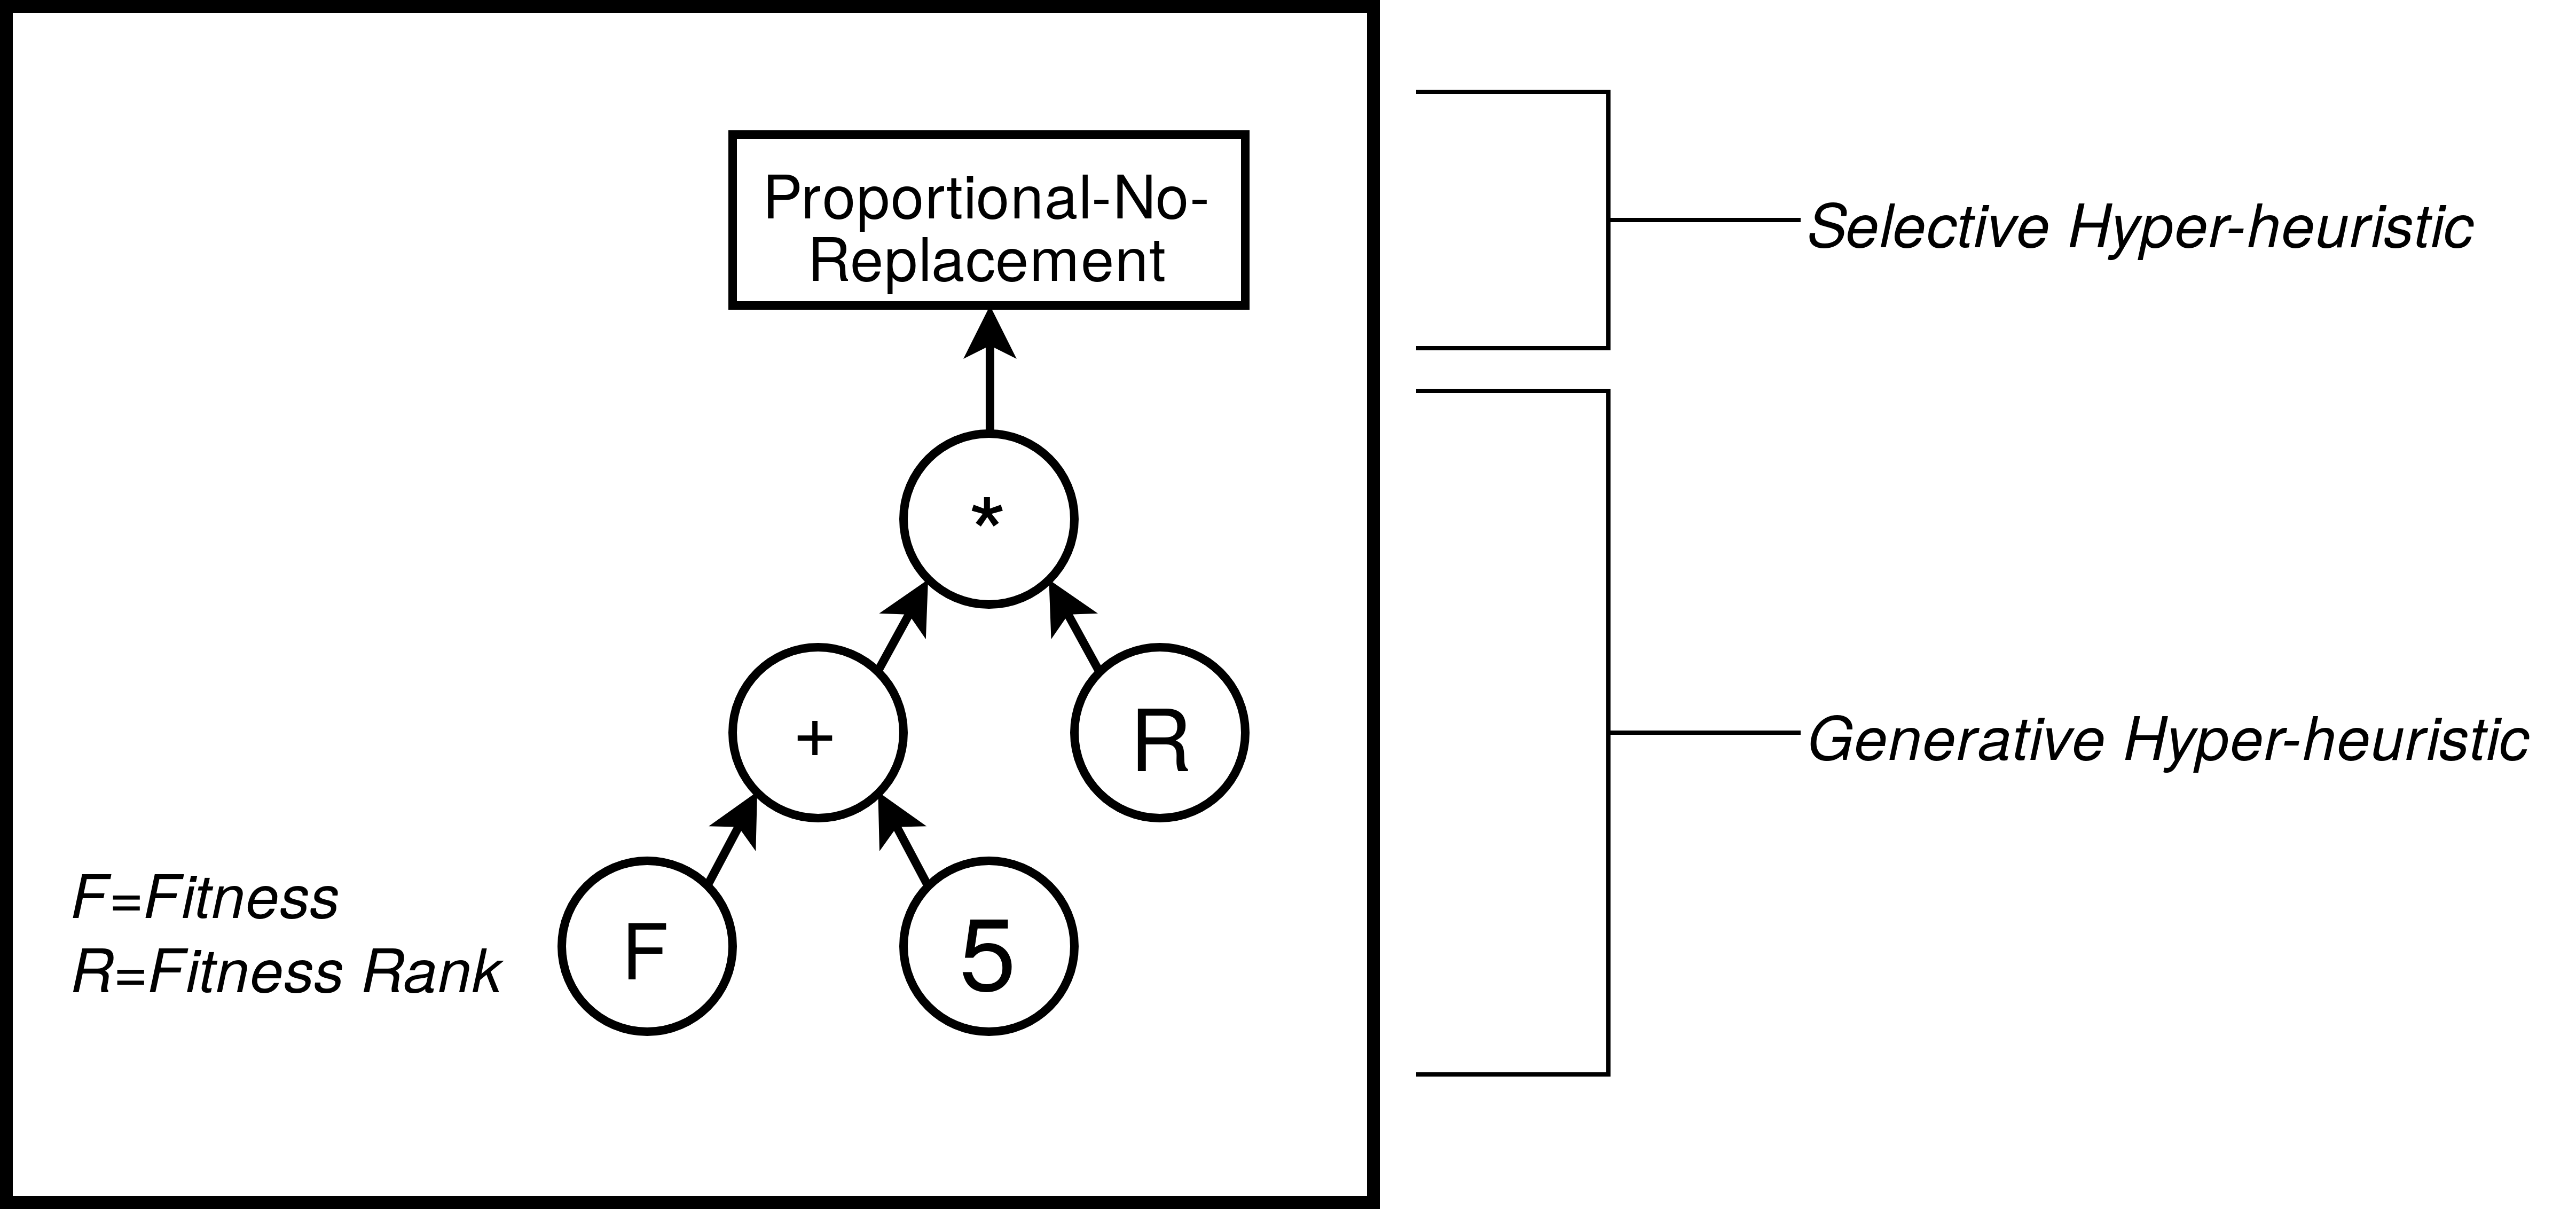
\includegraphics[width=0.45\textwidth]{example_eppsea}
	\caption{Example of a generated selection function.}
	\label{fig:example_adpsea}
\end{figure}

\begin{algorithm}
	\caption{An example of the pseudocode for a generated selection function. The function takes as input a population $P$ of individuals, and a number of individuals $m$ to be selected. Each individual $p$ in $P$ has member elements $p.Fitness$ and $p.FitnessRank$, encoding the individual's fitness and fitness ranking, respectively. Other generated selection functions may use additional information (see Table~\ref{tab:gp-terminals}).  The function returns a set of selected individuals. Note the weight calculation performed on Line~\ref{procline:gp-tree-line}, which is controlled by the GP-Tree encoded in the selection function. Also note that $\emptyset$ is used to denote the empty set.}
	\label{alg:ExampleSelection}
	\begin{algorithmic}[1]
		\Function {ExampleSelection}{$P, m$}
		\label{proc:ExampleSelection}
		\State $W(p) \leftarrow 0,\forall p \in P$
		\ForAll {$p \in P$}
		\State $W(p) \leftarrow (p.Fitness + 5)*p.FitnessRank$\label{procline:gp-tree-line}
		\EndFor
		\State $w_{min} \leftarrow minimum(W)$	
		\State $s \leftarrow 0$ 
		\ForAll {$w \in W$}
		\If {$w_{min}  < 0$}
		\State $s \leftarrow s + (w - w_{min} )$			
		\Else
		\State $s \leftarrow s + w$		
		\EndIf	
		\EndFor
		\State $selected \leftarrow \emptyset$
		\For {$j \leftarrow 1,m$}
		\State{$r \leftarrow random(0,s)$}
		\State $i \leftarrow 1$
		\State $p_s \leftarrow P(i)$
		\While {$r > W(p_s)$}
		\State $r \leftarrow r - W(p_s)$
		\State $i \leftarrow i + 1$
		\State $p_s \leftarrow P(i)$
		\EndWhile	
		\State $selected \leftarrow selected \cup p_s$
		\State $P \leftarrow P - p_s$
		\EndFor
		\State \Return $selected$
		\EndFunction
	\end{algorithmic}
\end{algorithm}

\begin{figure}
	\centering
	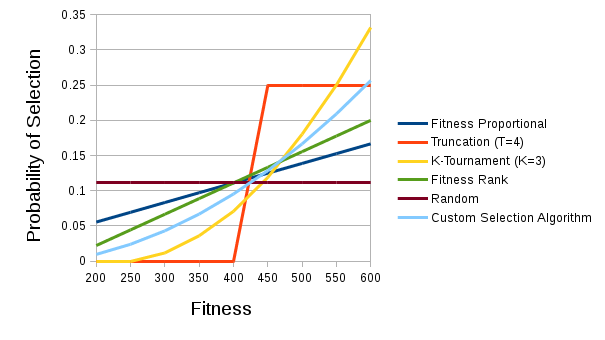
\includegraphics[width=0.5\textwidth]{selection_chances}
	\caption{A comparison of the chances that each member of a sample population, with fitnesses as listed, will be selected, under each of the typical selection strategies listed, as well as the custom selection strategy shown in Figure~\ref{fig:example_adpsea}.}
	\label{fig:selection_chances}
\end{figure}

\subsection{Search Methodology}
\label{Methodology-Search Methodology}

To develop high-quality selection functions, we need a method to search through the space of selection functions defined by the representation described in Section~\ref{Methodology-Encoding Selection Functions}. We use a meta-EA to develop the selection functions, treating each complete selection function as a member of a higher-order population. After generating an initial pool of randomly constructed selection functions, the quality of each complete selection function is determined, and well-performing selection functions are chosen to recombine and mutate into new candidate selection functions. 

The quality of each selection function is determined by running an underlying EA (CMA-ES) on a suite of static training instances from a benchmark function class. The underlying EA utilizes the selection function in question, and keeps all other parameters constant. The performance of the underlying EA is averaged over multiple runs, and is used to determine the quality of a selection function; selection functions that enable the EA to perform better, with all other parameters constant, are considered to be ``higher-quality'' selection functions. This information is fed back into the meta-EA to generate the next set of candidate selection functions. Selection functions that perform extremely poorly, because they fail to provide any selection pressure toward areas of high fitness, are pruned out of the population and never used to generate new selection functions. 

To prevent the size of the GP-Trees from growing too large, parsimony pressure is applied to the selection functions in the following manner: after the entire generation of selection functions is rated, the fitness assigned to each selection function is reduced by an amount equal to the number of nodes in the function's GP-Tree, times a parsimony coefficient $c$, times the difference in fitness between the best and worst selection functions in the population (after the extremely poor selection functions are removed). For example, suppose we have a population of three selection functions with the GP-Trees shown in Figure \ref{fig:parsimony_example}, and fitness assignments of 20, 20, and 30, respectively. For the first tree, the penalty due to parsimony pressure is calculated as $(best\ fitness - worst\ fitness) * c * size$. If we assume a parsimony coefficient of $c = 0.005$, then the fitness penalty is equal to $(30 - 20) * 0.005 * 5 = 10 * 0.025 = 0.25$, and the fitness assigned to the individual is $20 - 0.25 = 19.75$.

\begin{figure}
	\centering
	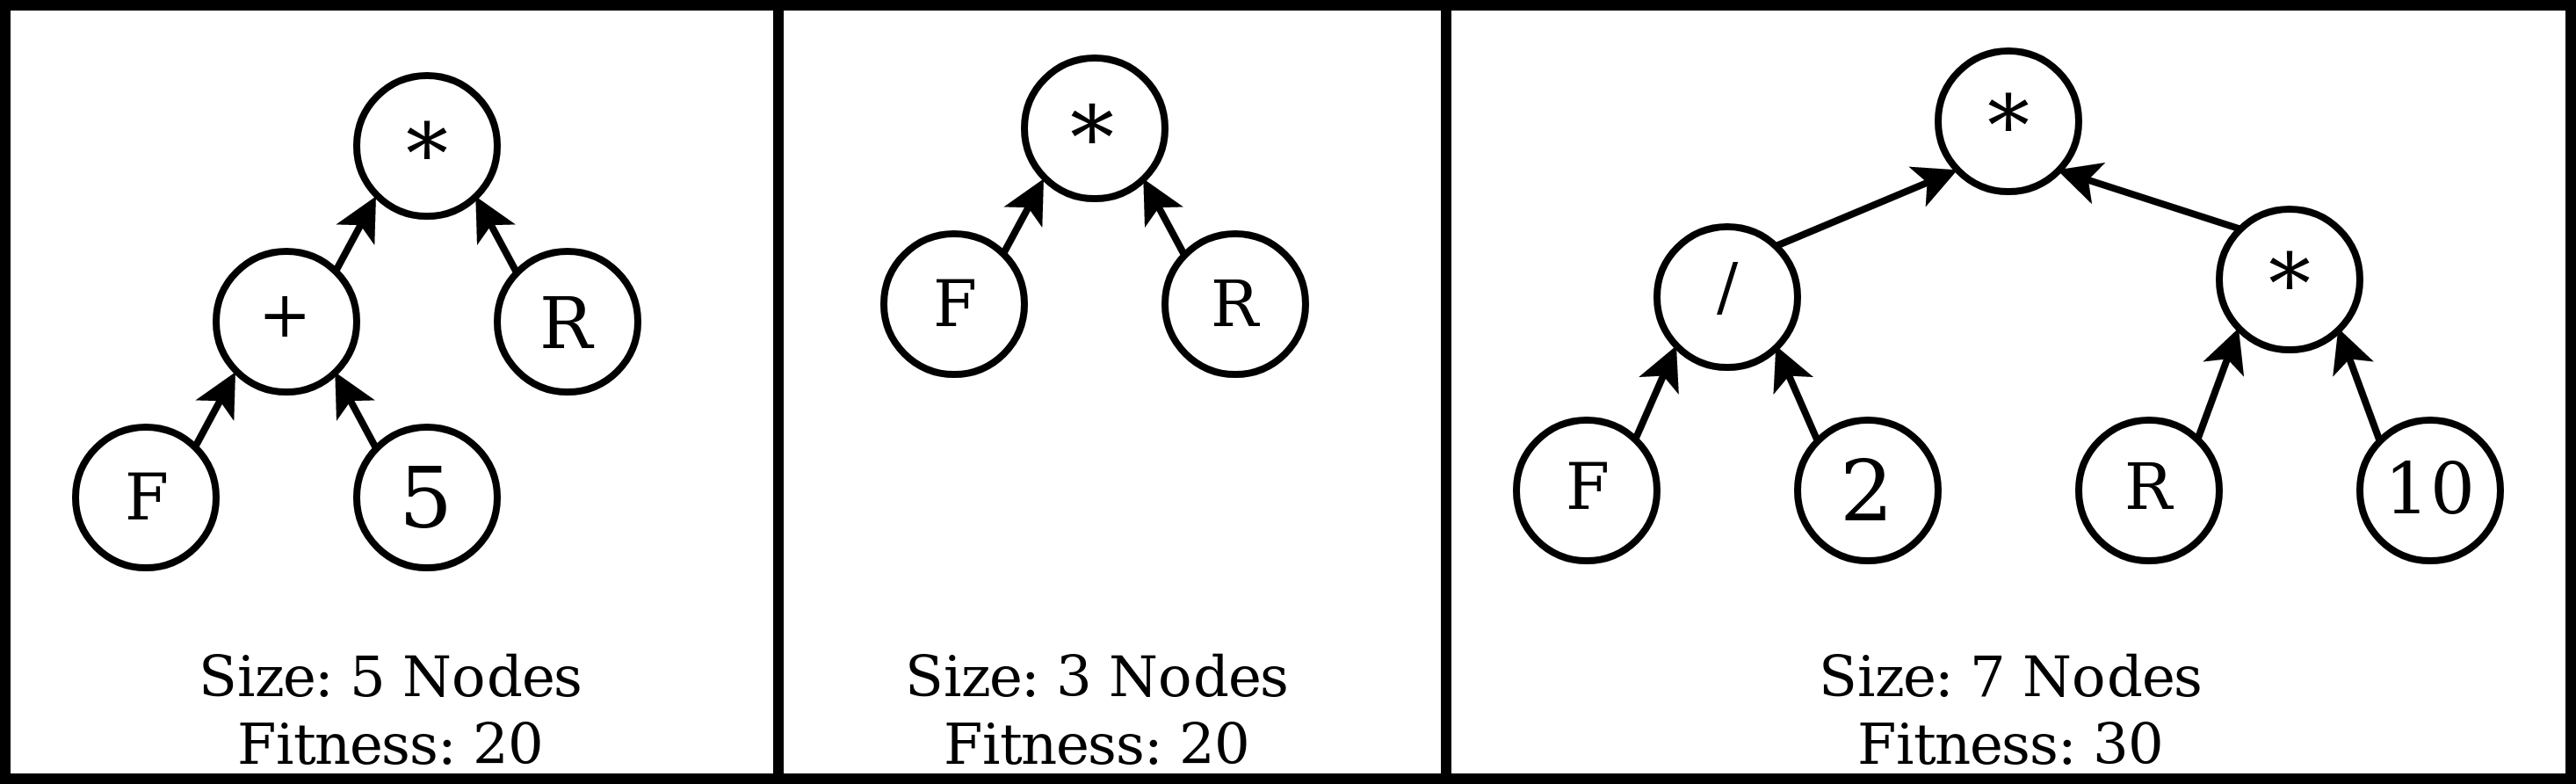
\includegraphics[width=0.5\textwidth]{parsimony_example}
	\caption{The GP-Trees for an example population of 3 individuals.}
	\label{fig:parsimony_example}
\end{figure}

When the meta-EA concludes, the bottom-level EA utilizing the best selection function from the meta-EA is run on a set of separate testing instances from the same function class to test the generalization of the selection function's performance. If the EA utilizing the best selection function performs significantly better on the testing instances than the same EA using a standard selection function, then we can say that the evolved selection function successfully generalized to the function class of interest. 

By using a meta-EA to evolve selection functions with \textit{a priori} computation, we are utilizing an offline hyper-heuristic, with the goal being to evolve a selection function that offers better generalized performance on all instances of a particular function class. For this initial exploration into evolving selection functions, we decided to employ an offline hyper-heuristic in order to better estimate the performance upper bound without the overhead potentially incurred by an online hyper-heuristic.

The benchmark function classes used for the underlying EA are selected from the Comparing Continuous Optimizers (COCO) platform used for the GECCO Workshops on Real-Parameter Black-Box Optimization Benchmarking~\citep{cocobbob}. This benchmark set provides a suite of real-valued optimization problems that serve as a robust testbed for optimization algorithms, including EAs. These functions are well-suited to measuring the strength of an EA and how well it performs under various conditions, which makes it an excellent choice for measuring how different selection functions impact the performance of an EA. Each function class is offered in multiple dimensionalities, and for each dimension, multiple unique instances of the function class are present. By using several different instances of a given problem for a given dimensionality, we can test whether an increase in performance offered by a higher-quality selection function generalizes to other instances within the function class. We do this by using only some of the instances during the meta-EA to evaluate the quality of selection functions, then run the bottom-level EA utilizing the evolved selection function on the unused, unseen instances. We select our benchmark problems from the 24 noiseless test function classes offered by the COCO platform.

\section{Experimental Setup}
\label{Primary Experiments}

The parameters for the meta-EA used in each experiment are shown in Table~\ref{tab:Meta-EA Parameters}. These parameters were manually tuned to allow for a population with high explorative potential while keeping the total computation time manageable.

\begin{table}
	\centering
	\caption{Meta-EA Parameters}
	\label{tab:Meta-EA Parameters}
	\begin{tabular}{c|c}
		\toprule
		Parameter& Value\\
		\midrule
		Population Size & 40 \\
		\hline
		Offspring Size & 40\\
		\hline
		Evaluation Count & 4000\\
		\hline
		Max GP-Tree Initialization Depth & 4\\
		\hline
		Parent Selection & \textit{k}-tournament, \textit{k}=4 \\
		\hline
		Survival Selection & Truncation\\
		\hline
		Mutation & Subtree Regeneration\\
		\hline
		Crossover & Subtree Crossover\\
		\hline
		Parsimony Pressure Coefficient & 0.0005\\
		\hline
		Mutation Rate & 0.25\\
		\hline
		Range for Constant Terminals & [-100, 100]\\
		\hline
		Range for Random Terminals & [-100, 100]\\
		\hline
		Number of Runs (Training) & 5 \\
		\hline
		Number of Runs (Testing) & 200\\
		
		\bottomrule
	\end{tabular}
\end{table}

To test our methodology, we target the CMA-ES algorithm for improvement. This algorithm repeatedly samples $\lambda$ points in a space around a mean, and uses a weighted combination of the high-value points to update the mean, as well as the parameters that control the shape of the space to be sampled in the next generation. In its traditional form, CMA-ES uses the $\mu$ highest-fitness points to update the mean; from an EA-perspective, this is akin to truncation selection. 

We used the meta-EA to evolve a new method of selecting which of the sampled points to use for recalculating the mean. The individuals of the meta-EA each encode a single selection function in their genome, which modifies the mean-update functionality of CMA-ES. Rather than selecting the $\mu$ highest-fitness points, which is done in standard CMA-ES, the encoded selection function selects a subset of all the sampled points, which are then ordered by fitness and used to update the mean. Once the mean is updated, all other state variables, such as the covariance matrix, are updated using the same methods as the unmodified CMA-ES.

To select benchmark functions for the CMA-ES, we use the 24 noiseless function classes in the COCO dataset. We use dimensionalities of 2, 3, 5, and 10, excluding 20 and 40 to save computational resources. The meta-EA is run separately for each combination of function class and dimensionality, using 6 of the instances for that function class and dimensionality to train the meta-EA and the rest of the available instances for testing generalization of the evolved selection function. For the parameters of CMA-ES, we use $\lambda=10 \times D$, $\mu = \lambda/2$, and $\sigma_i = 0.5$. The CMA-ES terminates on population convergence, after $10000 \times D$ evaluations, or after finding the solution to a function instance, as specified by the COCO benchmark platform.

When evaluating the performance of an evolved selection function to assign a fitness value to it, the fitness is taken as the proportion of the runs in which the modified CMA-ES reaches the global optimum, or moves close enough to it to meet the criteria to solve the function.

For each function instance in the testing set, we run the CMA-ES for 200 testing runs, both using the evolved selection function and unmodified. We then measure, for each testing instance, the proportion of runs which solved the function, in each case. 

\section{Results and Discussion}
\label{Results}

For each testing instance, the percentage of runs solved by the modified and unmodified CMA-ES is shown in Table~\ref{tab:experiment3Results}.

\begin{table*}
	\centering
	\caption{Percentage of Runs Solved By Modified CMA-ES/Unmodified CMA-ES, averaged over all instances}
	\label{tab:experiment3Results}
	\begin{tabular}{c|c|c|c|c}
		\toprule
		COCO Function Class & D=2 & D=3 & D=5 & D=10\\
		\midrule
		1 &  100.0\% / 100.0\%  &  100.0\% / 100.0\%  &  100.0\% / 100.0\%  &  100.0\% / 100.0\% \\
		\hline
		2 &  100.0\% / 100.0\%  &  100.0\% / 100.0\%  &  100.0\% / 100.0\%  &  100.0\% / 100.0\% \\
		\hline				
		3 &  35.65\% / 34.2\%  &  22.0\% / 21.35\%  &  7.6\% / 6.6\%  &  1.2\% / 1.35\% \\
		\hline
		4 &  32.15\% / 3.3\%  &  0.15\% / 0.25\%  &  0.0\% / 0.0\%  &  0.0\% / 0.0\% \\
		\hline
		5 &  100.0\% / 100.0\%  &  100.0\% / 100.0\%  &  100.0\% / 100.0\%  &  100.0\% / 100.0\% \\
		\hline		
		6 &  100.0\% / 100.0\%  &  100.0\% / 100.0\%  &  99.1\% / 100.0\%  &  96.0\% / 0.0\% \\
		\hline
		7 &  98.05\% / 94.35\%  &  100.0\% / 97.65\%  &  99.35\% / 99.4\%  &  100.0\% / 99.95\% \\
		\hline
		8 &  99.85\% / 100.0\%  &  100.0\% / 100.0\%  &  99.9\% / 99.5\%  &  99.8\% / 100.0\% \\
		\hline				
		9 &  100.0\% / 100.0\%  &  100.0\% / 100.0\%  &  100.0\% / 100.0\%  &  100.0\% / 100.0\% \\
		\hline
		10 &  100.0\% / 100.0\%  &  100.0\% / 100.0\%  &  100.0\% / 100.0\%  &  100.0\% / 100.0\% \\
		\hline	
		11 &  100.0\% / 100.0\%  &  100.0\% / 100.0\%  &  100.0\% / 100.0\%  &  100.0\% / 100.0\% \\
		\hline					
		12 &  99.55\% / 100.0\%  &  99.5\% / 100.0\%  &  99.85\% / 100.0\%  &  100.0\% / 44.05\% \\
		\hline
		13 &  100.0\% / 100.0\%  &  100.0\% / 100.0\%  &  100.0\% / 100.0\%  &  100.0\% / 100.0\% \\
		\hline
		14 &  100.0\% / 100.0\%  &  100.0\% / 100.0\%  &  100.0\% / 100.0\%  &  100.0\% / 100.0\% \\
		\hline				
		15 &  41.45\% / 41.95\%  &  32.85\% / 32.45\%  &  24.55\% / 24.0\%  &  11.95\% / 16.85\% \\
		\hline
		16 &  65.7\% / 65.65\%  &  59.95\% / 64.0\%  &  58.2\% / 57.1\%  &  40.05\% / 39.7\% \\
		\hline
		17 &  96.05\% / 75.0\%  &  96.15\% / 81.9\%  &  96.7\% / 94.6\%  &  99.2\% / 99.2\% \\
		\hline
		18 &  96.85\% / 64.05\%  &  97.6\% / 79.25\%  &  93.5\% / 91.75\%  &  93.9\% / 94.9\% \\
		\hline				
		19 &  55.05\% / 36.1\%  &  20.1\% / 20.9\%  &  6.85\% / 5.8\%  &  6.6\% / 0.45\% \\
		\hline
		20 &  48.35\% / 24.8\%  &  19.35\% / 12.15\%  &  2.25\% / 1.5\%  &  0.0\% / 0.0\% \\
		\hline
		21 &  56.8\% / 27.65\%  &  55.4\% / 28.7\%  &  36.05\% / 23.3\%  &  28.6\% / 36.0\% \\
		\hline
		22 &  47.15\% / 35.25\%  &  25.8\% / 27.85\%  &  14.2\% / 12.75\%  &  5.95\% / 0.4\% \\
		\hline		
		23 &  70.35\% / 73.3\%  &  54.7\% / 52.3\%  &  32.05\% / 31.2\%  &  7.35\% / 8.05\% \\
		\hline
		24 &  1.6\% / 1.45\%  &  0.1\% / 0.3\%  &  0.0\% / 0.0\%  &  0.0\% / 0.0\% \\

		\bottomrule
	\end{tabular}
\end{table*}

For the function classes 4, 6, 12, 17, 18, 19, 20, and 21, the CMA-ES modified with the evolved selection function solved the function instances at least 20 percent more often than the unmodified CMA-ES for at least one dimensionality. For the function classes 4 and 19, the success rate of CMA-ES increased by 20-30 percent when modified with the evolved selection function at $D=2$, but performed similarly to the unmodified CMA-ES at other dimensionalities. For function classes 20 and 21, a performance increase is seen on dimensionalities $D=2, 3,$ and $5$, but not $D=10$; curiously, the modified CMA-ES performs worse on function class 21 when $D=10$. For function classes 17 and 18, performance increases are seen for $D=2$ and $D=3$, with negligible performance differences on the other dimensionalities. Function class 22 sees about a 12 percent increase in solution rate on $D=2$, but negligible improvement for other dimensionalities. For function classes 6 and 12, performance is similar for $D=2, 3,$ and $5$, but for $D=10$, there is a significant performance increase: on function 6, the success rate increased from 0 percent to around 96 percent, and on function class 12, the success rate increased from 18-67 percent, varying across the function instances, to 100 percent for all function instances.

For the other function classes, there was no major difference between the success rate of the modified and unmodified CMA-ES. In a few cases, the modified CMA-ES performs marginally worse than the unmodified CMA-ES, but the difference in solution rate usually no more than 5 percent, and only 7.4 percent at most.

\subsection{Discussion of Results}
\label{resultsDiscussion}

We observed that evolving a new selection function for CMA-ES increased its solution quality on 6 of the 11 functions tested. In particular, we observed two cases with high dramatic improvements: the tests for COCO function classes 6 and 12 for dimensionality $D=10$. In the case of function class 6, the unmodified CMA-ES was unable to solve any of the testing instances, but the CMA-ES using the evolved selection solved these instances nearly 100\% of the time. In the case of function class 12, the success rate of the unmodified CMA-ES varied strongly between instances, ranging from 18 to 67\%, with an average success rate of 44.05\% across all instances. The modified CMA-ES, however, solved every test instance, reaching the global best fitness in each of 200 runs, on each of the testing instances, achieving a 100\% success rate. By observing the increases in success rate for some of the functions, it is clear that evolving a new selection scheme for CMA-ES provides a substantial benefit in some cases. 

The five cases where no improvement was observed involved functions that were highly multimodal. Three of these function were variants of the Rastrigin function, a highly multimodal function and the other two---the Weierstrass Function and the Katsuura Function---are highly rugged. It is likely, in these cases, that CMA-ES requires some other improvement aside from a new selection scheme to better learn and traverse the global structures of these functions. Because we only replaced the selection scheme of CMA-ES, we only changed how it internally updates the mean. Improving the performance of CMA-ES on these functions likely requires more intelligent updating of the other internal variables of CMA-ES, such as the evolution paths, the covariance matrix, and the step size.

$F=21$, $D=10$ is the one case tested where CMA-ES performed markedly worse than unmodified CMA-ES. This effect is likely due to overspecialization to the set of training instances.

\section{Conclusions}
\label{Conclusion}
We hypothesized that a hyper-heuristic search through the space of selection functions for EAs could improve the performance of an EA on a particular function class by discovering a specialized selection function. We developed a representation of selection functions that uses a Koza-style GP-Tree to relate an individual's fitness value and fitness ranking to its relative probability of selection, and used a meta-EA to search through the space of selection functions in this representation. 

With this meta-EA, we have shown that it is possible to generate new selection functions, tuned to a particular benchmark function, that can enable an EA to significantly outperform conventional selection functions on those functions. Thus, we show that, in order to discover the optimum selection method for an EA operating on a particular function, it may not be sufficient to use any of the static conventional selection functions tested. We have also shown that, in some cases, this performance increase from a custom selection algorithm will generalize to similar functions in the same function class. Therefore, if one expects to run the same EA on many functions from the same function class, one might expect to gain a performance increase by doing some \textit{a priori} calculation to develop a specialized selection algorithm trained on instances of that function class, which would then enable an EA utilizing that selection function to perform better on other instances of that function class. However, our experiments have also shown that, for certain functions, replacing only the selection function may not yield significant performance improvements, depending on the behavior of the search strategy and the nature of the function being optimized by the EA. Careful consideration must be given to determine what the effect of tuning the selection scheme of a given EA will be on the performance of that EA, and whether such tuning will cause the EA to have an appreciable performance increase on the function class in question. 

\subsection{Threats To Validity}
\label{Threats to Validity}
Although we strove to ensure the robustness of our methodology and experimental setup, there are some careful considerations that must be made when interpreting these results which may threaten the validity of our claims.

Of obvious note is the fact that, while we have shown improved performance on the benchmark functions tested, we still have yet to test this method on EAs run in real-world scenarios, and we do not yet know whether the supposed performance benefit is, in practice, enough to warrant the \textit{a priori} computation necessitated by our methods.

We chose CMA-ES as a testing target for extending our method to a more state-of-the-art method. However, the implementation of CMA-ES we used was fairly basic, lacking restarts in particular, and much research has been done on improved and alternative variants of CMA-ES. For certain problems, these newer variants may offer the same, or greater, performance increases as an evolved selection function. However, if these newer variants also use some selection function to update internal variables, as the basic implementation does, then evolving a new selection function for these newer variants could generate an even greater increase in performance; this opens up an avenue for future research.

\subsection{Future Work}
\label{Future Work}
The work presented in this paper opens a number of potential avenues for future research. Of primary concern is the fact that the meta-EA presented in this paper requires a large amount of \textit{a priori} computation to generate a high-quality selection function. While this computational cost may be worth it for EAs that will run on functions from the same function class many times, a more efficient method of finding good selection functions has a much greater potential to benefit EAs in general. Exploring a method of online learning could allow for the elimination of the expensive \textit{a priori} computation time, allowing specialized selection functions to be generated during the evolution.

The CMA-ES in our experiments was tuned to increase performance on the COCO benchmark function classes. While these functions are difficult and non-trivial to optimize for, they are entirely artificial, and the meta-EA has not yet been used to tune an EA for solving a real-world function class. A major next step for this work is to apply the meta-EA to real-world EAs that could benefit from new, specialized selection functions. Of particular interest are EAs that are expected to be run many times on functions from the same general function class, which would, over many runs, amortize the \textit{a priori} computation time required to tune the selection function.

Because the objective of this paper is similar to the work done to develop selection algorithms via Grammatical Evolution~\citep{lourencco2013selection} and register machines~\citep{woodward2011selection}, it remains to be seen which cases each method is more effective for, and a direct comparison of the methods on the same benchmark functions may yield more insight into which offers better performance benefits under certain conditions.

The framework of CMA-ES used was fairly basic, lacking features such as restarts. In addition, many techniques have been developed to improve the performance of CMA-ES on functions where it may be deficient, such as in $(1+1)$-CMA-ES~\citep{igel2006cmaes1plus1} and the Active CMA-ES~\citep{jastrebski2006activecmaes}. Evolving a specialized selection function for these new forms of CMA-ES may lead to even greater performance gains, or may not even be necessary for particular es. Additionally, as we noted in our conclusions, we only made efforts to improve the selection of points used in the mean-update step of CMA-ES, which allowed to it gain increased performance in some, but not all, of the problem cases tested. Further experiments to tune the selection of points used for updating the other internal variables, such as evolution path, covariance matrix, and step-size, may lead to greater changes in the behavior of CMA-ES, and thus, greater changes in performance.

For our meta-EA, the GP-Trees utilized several terminals related to the individual, such as fitness, fitness ranking, uniqueness of genome, and birth generation, as well as terminals related to the evolution at large, such as population size and generation number. Adding additional available terminals increases the information available to the meta-EA, allowing it to potentially evolve more intelligent selection functions. In particular, there are no terminals that allow the selection function to have any internal persisting memory from generation to generation, such as the best fitness of past generations or which individuals have been selected previously. Additionally for EA's with sexual reproduction, or selection schemes involving individuals selected in pairs or groups, there is no terminal that measures two individuals relative to each other. This prevents the meta-EA from developing a selection function based on any information about an individual's mate, such as fitness, genome, etc. To add these terminals to the meta-EA, the selection function representation would need to be updated such that, when determining the desirability of an individual, the GP-Tree would take as input the information of some other individual to be selected for a similar purpose, such as recombination of the same child (for an EA with two-parent recombination) or selection for update of the same internal variable (for an Evolution Strategy such as CMA-ES).

The parameters at the meta-EA level were manually tuned to allow for a high degree of exploration. A sensitivity analysis of these parameters, as well an investigation of parameter tuning/control, could lead to increased performance of the meta-EA.

\bibliographystyle{spbasic}
\bibliography{eppsea_GECCO2019_bibliography}

% For one-column wide figures use
%\begin{figure}
% Use the relevant command to insert your figure file.
% For example, with the graphicx package use
%  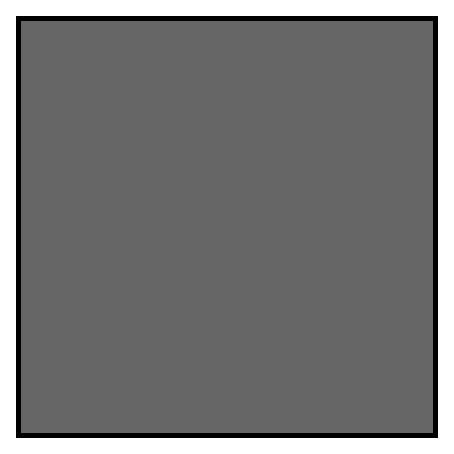
\includegraphics{example.eps}
% figure caption is below the figure
%\caption{Please write your figure caption here}
%\label{fig:1}       % Give a unique label
%\end{figure}
%
% For two-column wide figures use
%\begin{figure*}
% Use the relevant command to insert your figure file.
% For example, with the graphicx package use
%  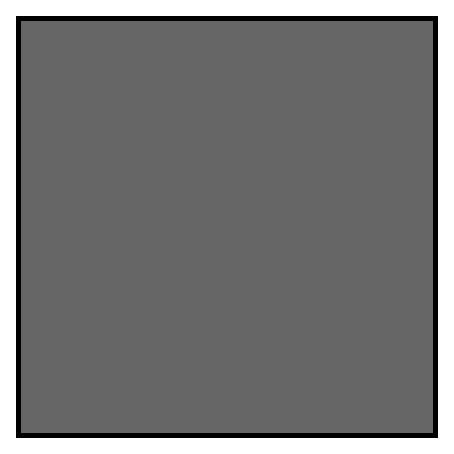
\includegraphics[width=0.75\textwidth]{example.eps}
% figure caption is below the figure
%\caption{Please write your figure caption here}
%\label{fig:2}       % Give a unique label
%\end{figure*}
%
% For tables use
%\begin{table}
% table caption is above the table
%\caption{Please write your table caption here}
%\label{tab:1}       % Give a unique label
% For LaTeX tables use
%\begin{tabular}{lll}
%\hline\noalign{\smallskip}
%first & second & third  \\
%\noalign{\smallskip}\hline\noalign{\smallskip}
%number & number & number \\
%number & number & number \\
%\noalign{\smallskip}\hline
%\end{tabular}
%\end{table}


%\begin{acknowledgements}
%If you'd like to thank anyone, place your comments here
%and remove the percent signs.
%\end{acknowledgements}


% Authors must disclose all relationships or interests that 
% could have direct or potential influence or impart bias on 
% the work: 
%
% \section*{Conflict of interest}
%
% The authors declare that they have no conflict of interest.


% BibTeX users please use one of
%\bibliographystyle{spbasic}      % basic style, author-year citations
%\bibliographystyle{spmpsci}      % mathematics and physical sciences
%\bibliographystyle{spphys}       % APS-like style for physics
%\bibliography{}   % name your BibTeX data base

% Non-BibTeX users please use
%\begin{thebibliography}{}
%
% and use \bibitem to create references. Consult the Instructions
% for authors for reference list style.
%
%\bibitem{RefJ}
% Format for Journal Reference
%Author, Article title, Journal, Volume, page numbers (year)
% Format for books
%\bibitem{RefB}
%Author, Book title, page numbers. Publisher, place (year)
% etc
%\end{thebibliography}
\end{document}
% end of file template.tex

